\subsection{Initial Software Analysis}
This section will cover our initial analysis of the requirements as given in the project description [reference: project description]. We will describe different RUP artifacts created during the process, such as Use Cases, Domain Model, System Sequence Diagrams and Supplementary Requirements.\\
Please note that in the spirit of agile development, the artifacts created in the first sprints were incomplete and draft-like in appearance. The artifacts are then extended and reviewed in later iterations as the need for understanding them increases.\\
\subsubsection{Domain Model and Relational Model}
Before doing any design of the system, we realized the need for a common terminology to describe our understanding of file-sharing and document handling applications. We made a crude initial domain model and discussed our understanding of each entity:\\
\begin{figure}[H]
  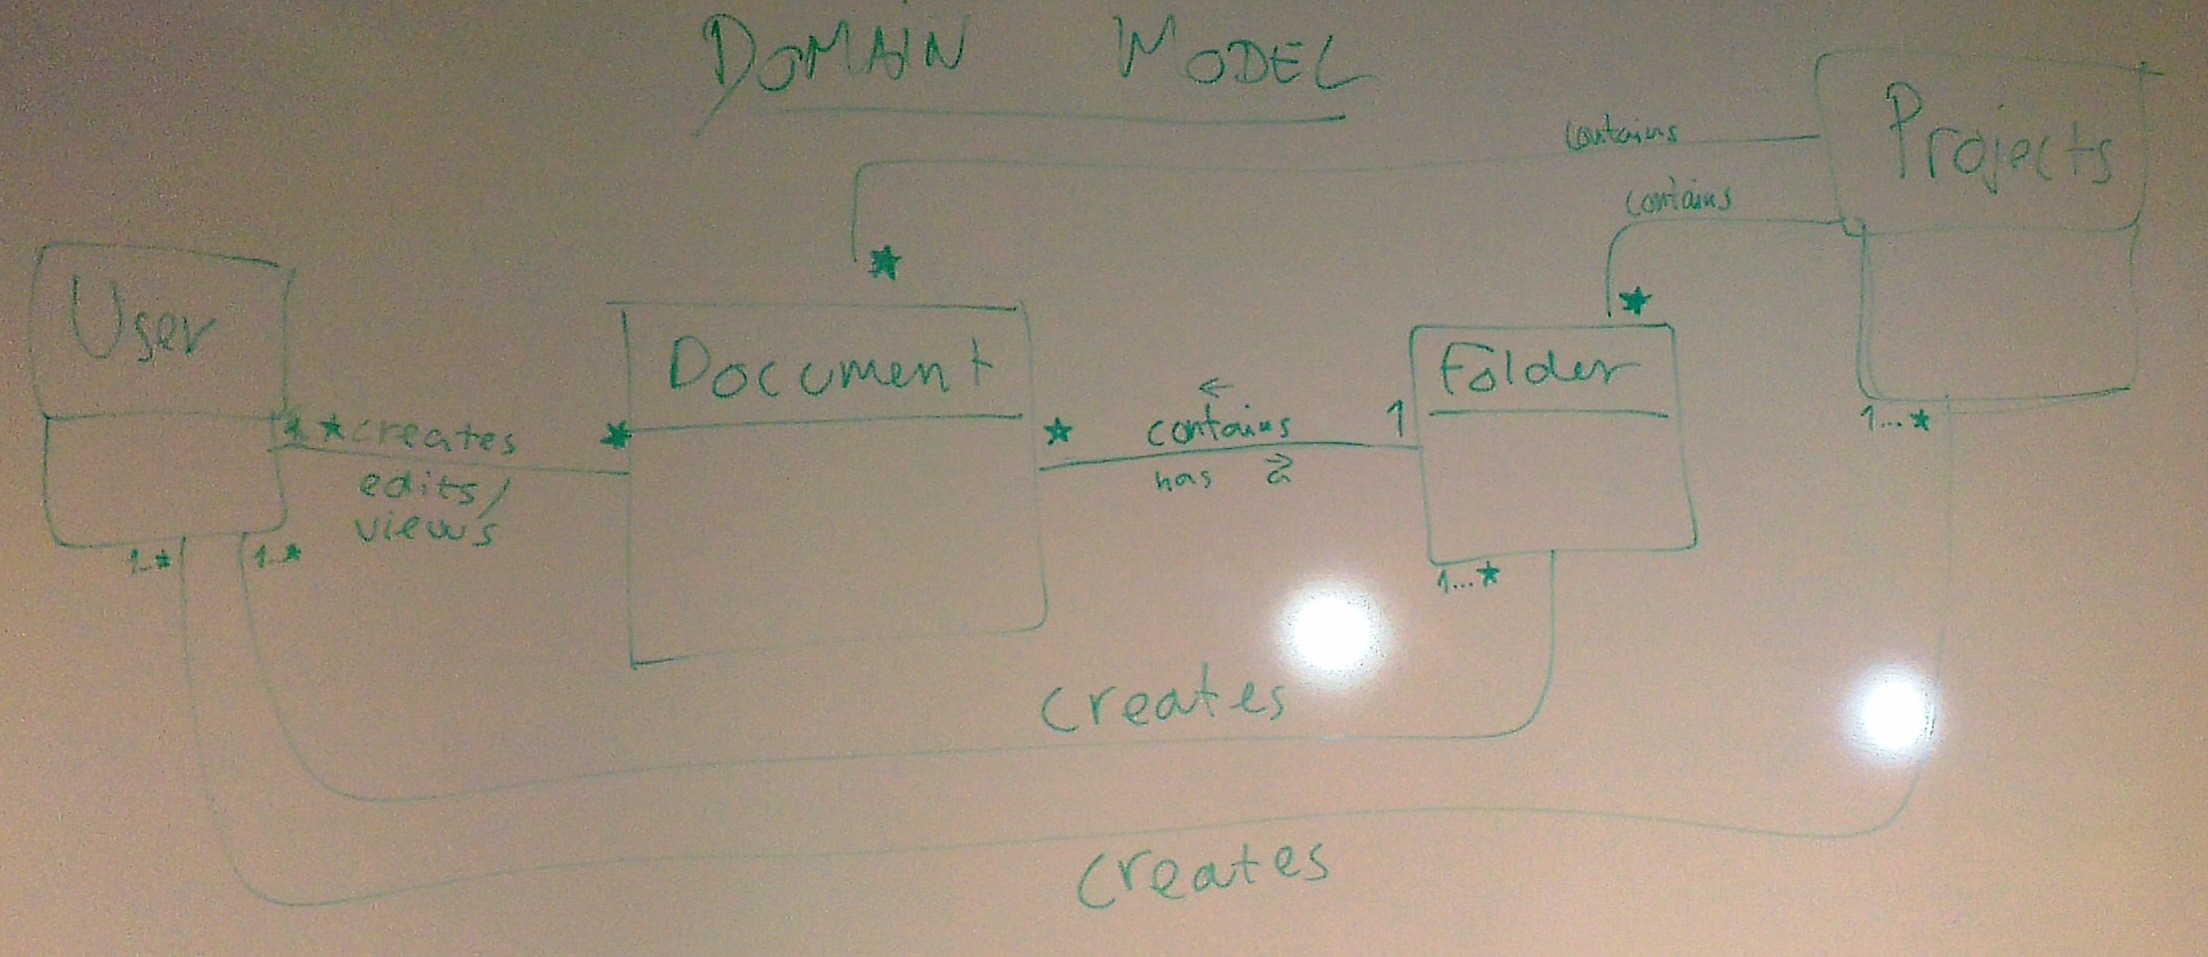
\includegraphics[width=\textwidth,natwidth=2208,natheight=957]{illustrations/DomainModel.jpg}
  \caption{Domain Model}
  \label{domainmodel}
\end{figure}
The picture shows our first draft of the domain model. It shows that our domain model reflects the entities needed to fulfill the requirements given in the project description.\\
Additionally, we quickly identified that online storage using a database would be an important part of our system. Therefore, we added a relational data model to create a better view of the entities in this aspect:\\
\begin{figure}[H]
  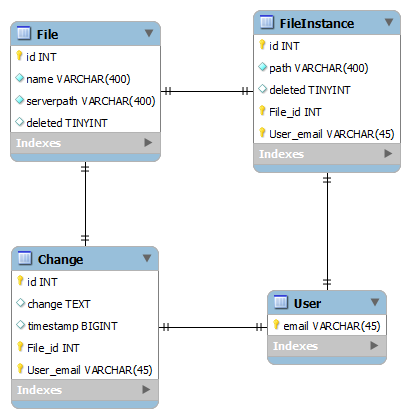
\includegraphics[width=\textwidth,natwidth=410,natheight=418]{illustrations/RelationalData-model.png}
  \caption{Relational Data-Model}
  \label{relationalmodel}
\end{figure}
As it clearly shows, both of these models were quickly drawn and used primarily for their discussion value. The relational model also covers changes made to a document, which we did not include in the initial domain model.\\
Later, we'll review both models as they are expanded to support the requirements.\\
\subsubsection{Requirements Analysis with Use Cases}
Before defining any requirements, a reasonable exercise could be to create a vision for the product to develop \cite[p.~58]{OOAD}. However, as the high level requirements were already defined in the project description, we've decided to skip this artifact.\\
\newline
Understanding the requirements means creating different artifacts that helps develop early ideas of how to solve each requirement. We wrote down several use cases in a brief form, only covering 1) the goal of the use case and 2) brief explanations of scenarios. A few of the use cases were expanded to include an extended description of alternate case flows as well as pre- and postconditions. Below is an example of a brief use case, ViewVersionHistory:\\
\newline
% [UseCase #4 here in cursive as a quote and delete it from appendix].  
\texttt{USE CASE \#4: VIEW VERSION HISTORY\\
The user wants to view a history for a file in the Slice Of Pie system. He will select a file from the graphical user interface in the system and click on a show version history button. The system will retrieve version history for the file and display it in a new window. \\
ALTERNATE:\\
The user wants to revert document to an earlier state. This use case has yet to be defined and elaborated on.}\\
% Margin?
\newline
The example shows a Use Case detailing the process of viewing a version history of a file.
The use cases created in this sprint are shown in [Appendix, Use Cases page \pageref{usecases}].
% ref
\subsubsection{Non-trivial requirements}
To further elaborate on requirements that are complicated to implement in the system, we've created additional artifacts to understand them. The example we're gonna show here is the users ability to synchronize documents between a client and the server holding the documents in online storage. To illustrate the interaction between the user and the system when this process is occurring, a System Sequence Diagram is drawn to display this [reference to Appendix: SSD2 (Synchronize)]. The SSD is shown in the Appendix.\\
% !! -- add ref
Moreover, to elaborate on the conditions of the requirement, we've created a Operation Contract as shown below (show in quotes?):\\
% !! -- includes note
\begin{table*}[ht]\centering
  \ra{1.3}
  \begin{tabularx}{\textwidth}{@{}rXXl@{}}\toprule
    \textbf{Contract CO1:} & SynchronizeWithServer (Make sure name is same\\
    \textbf{Cross References:} & Use Case \#2: Synchronize\\
    \textbf{Preconditions:} &  The user has an internet connection. The server is up and running.\\
    \textbf{Postconditions:} & The user has received files made in another client application.\\
    & The client has sent files to online storage.\\
    & The user interface displays the newly received files.\\
    \bottomrule
  \end{tabularx}
\end{table*}
The artifacts described above serves to make the requirement explicit and well-defined. The requirement is purely functional, however, and does not specify any measurable quality factors on the Use Case such as: how fast the process should be, how we should handle errors etc. However, trying to elaborate on all requirements is a time-consuming process and as RUP suggests \cite[12.2 p.~196]{OOAD}, we'd rather start implementing the high-risk elements of the requirements, reviewing and adapting the requirements at a later time. \\
\subsubsection{Supplementary Specification}
As part of the initial analysis, it is suggested by RUP that a coarse supplementary specification is started in the inception of the iterative development \cite[7.1 p.~102]{OOAD}. Hence, we created an outline of the non-functional requirements in a Supplementary Specification. The non-functional requirement is presented as the FURPS+ checklist. The main reason for this specification is the impact the non-functional requirements may have on the logical architecture of the system.\\
\newline
The Supplementary Specification concludes our artifacts created as part of the initial analysis. These artifacts are mainly supposed to provide a base for our initial code design and choice of logical architecture.\\